% ---------------------------------------------------------------------------
\section{Model Development and Evaluation}
\label{sec:models}
% ---------------------------------------------------------------------------

\subsection{Validation design}

All eight families are evaluated on identical folds, features and preprocessing, so
that differences in error are attributable to the estimator. The protocol is
five-fold cross-validation with shuffling and seed 42, producing one out-of-fold
prediction for each of the 1,458 transactions. Preprocessing is fitted inside each
fold as part of the scikit-learn pipeline \citep{pedregosa2011sklearn}, so imputation
and scaling statistics are computed without the validation rows, and the same
pipeline object is later serialised for serving.

Hyperparameters are tuned inside the cross-validation loop. The three regularised
linear models use exhaustive grid search over their penalty paths: eight values of
$\alpha$ for ridge and lasso and eighteen combinations of $\alpha$ and the $L_1$
ratio for the elastic net \citep{tibshirani1996lasso,zou2005elasticnet}. The four
tree ensembles use randomised search, which is more efficient than a grid when only a
few hyperparameters matter \citep{bergstra2012random}: 14 draws for the random
forest, 10 for gradient boosting, 22 for XGBoost and 30 for LightGBM
\citep{chen2016xgboost,ke2017lightgbm}. The selection rule is the lowest out-of-fold
root mean squared error in log space; business metrics are reported alongside but do
not influence selection. Selecting on the same out-of-fold predictions that are then
reported is optimistically biased \citep{varma2006bias}, which is why the temporal
holdout of Section~\ref{sec:models} is treated as the independent check.

\subsection{Benchmark of eight regression families}

Table~\ref{tab:benchmark} presents the results. The regularised linear models occupy
the first four places. The elastic net is selected with an out-of-fold RMSE of 20,019
\USD, a mean absolute error of 13,537 \USD{} and an $R^2$ of 0.9365; lasso is 3.6
\USD{} behind in root mean squared error, a difference far below any meaningful
threshold that should be read as a tie between the two sparse linear specifications.
Ridge and ordinary least squares follow at 20,172 and 21,135 \USD. The boosted
ensembles reach 22,471 \USD{} (XGBoost), 22,518 \USD{} (LightGBM) and 22,689 \USD{}
(gradient boosting), and the random forest is last at 25,725 \USD.

\begin{table}[htbp]
\centering
\caption{Out-of-fold performance of the eight regression families under identical
five-fold cross-validation. The selected model is shown in bold. Dollar figures are
in \USD; the tolerance column is the share of estimates within $\pm$15,000 \USD{} of
the realised price.}
\label{tab:benchmark}
\small
\begin{tabular}{@{}lrrrrrr@{}}
\toprule
\textbf{Model} & \textbf{RMSE} & \textbf{MAE} & \textbf{MAPE} & \textbf{$R^2$} & \textbf{Within} & \textbf{Cost} \\
 & & & (\%) & & \textbf{15k (\%)} & (\USD) \\
\midrule
\textbf{Elastic net} & \textbf{20,019} & \textbf{13,537} & \textbf{7.98} & \textbf{0.9365} & \textbf{69.7} & \textbf{16,708} \\
Lasso & 20,023 & 13,625 & 8.02 & 0.9365 & 69.5 & 16,848 \\
Ridge & 20,172 & 13,753 & 8.13 & 0.9356 & 69.3 & 17,005 \\
Linear regression & 21,135 & 14,500 & 8.56 & 0.9293 & 65.8 & 18,009 \\
XGBoost & 22,471 & 14,419 & 8.25 & 0.9200 & 68.3 & 17,564 \\
LightGBM & 22,518 & 14,665 & 8.49 & 0.9197 & 66.5 & 17,964 \\
Gradient boosting & 22,689 & 14,674 & 8.49 & 0.9185 & 65.9 & 17,925 \\
Random forest & 25,725 & 15,803 & 9.02 & 0.8952 & 66.5 & 18,923 \\
\bottomrule
\end{tabular}
\end{table}

The result is informative rather than surprising. With a log-transformed target and
a feature set whose main effects are strong and largely additive, a well-regularised
linear model has little bias left to remove, while a tree ensemble pays a variance
price for interactions the sample cannot support \citep{hastie2009esl}. The random
forest is worst by a clear margin: averaging many deep trees smooths the prediction
surface and cannot extrapolate beyond the range of the training target, which
penalises exactly the expensive properties the residual analysis identifies as
difficult. The ranking by mean asymmetric cost is not identical to the ranking by
RMSE, because XGBoost over-values less often than linear regression, but the elastic
net still has the lowest cost of the eight.

The selected estimator combines an $L_1$ penalty, which sparsifies, with an $L_2$
penalty, which stabilises correlated features \citep{zou2005elasticnet}. Its largest
standardised coefficients belong to the infrequent-zoning indicator ($-0.268$), rooms
above grade ($0.072$), the infrequent-functional indicator ($-0.071$), the Crawford
neighbourhood ($0.068$), the quality--condition index ($0.057$) and total floor area
($0.056$). A coefficient on a rare indicator applies to few rows and reflects the
composition of that group rather than a general mechanism, which is why the
discussion of drivers relies on SHAP rather than on raw coefficients.

\subsection{Calibrated prediction intervals}

Point estimates alone are insufficient, because the platform must know when to
publish a valuation and when to escalate it. Intervals are produced by split
conformal prediction \citep{angelopoulos2023conformal}: the absolute residuals of the
out-of-fold predictions in log space are collected and the quantile at level
$\lceil (n+1)(1-\alpha)\rceil/n$ is computed, which provides finite-sample marginal
coverage under exchangeability. The quantiles are 0.1173 log points at the 80 per
cent level and 0.1648 at the 90 per cent level, and the interval is obtained by
adding and subtracting the quantile in log space before back-transforming, which
makes it multiplicative and approximately proportional in dollars.

Table~\ref{tab:coverage} reports empirical coverage. Overall coverage is 0.801 and
0.901 at the two nominal levels, as close to exact as a sample of this size allows.
The segment results are less comfortable: the entry band is covered at 0.718 against
a nominal 0.80, a shortfall of 8.2 percentage points, and the luxury band at 0.783;
at the 90 per cent level the entry band reaches 0.833 and the luxury band 0.870. The
mid and upper bands are over-covered. Interval widths are stable at 23.7 per cent of
the estimate for the 80 per cent interval and 33.3 per cent for the 90 per cent
interval.

\begin{table}[htbp]
\centering
\caption{Empirical coverage of the split-conformal intervals, overall and by price
band, computed on the out-of-fold predictions used for calibration. A negative gap
means the interval covers fewer sales than its nominal level.}
\label{tab:coverage}
\small
\begin{tabular}{@{}llrrr@{}}
\toprule
\textbf{Level} & \textbf{Segment} & \textbf{Coverage} & \textbf{Gap} & \textbf{Mean width (\% of price)} \\
\midrule
80\% & All & 0.801 & $+0.001$ & 23.7 \\
80\% & Entry ($<$130k) & 0.718 & $-0.082$ & 24.6 \\
80\% & Mid (130k--200k) & 0.836 & $+0.036$ & 23.5 \\
80\% & Upper (200k--300k) & 0.831 & $+0.031$ & 23.3 \\
80\% & Luxury ($\geq$300k) & 0.783 & $-0.017$ & 22.6 \\
90\% & All & 0.901 & $+0.001$ & 33.3 \\
90\% & Entry ($<$130k) & 0.833 & $-0.067$ & 34.7 \\
90\% & Mid (130k--200k) & 0.941 & $+0.041$ & 33.1 \\
90\% & Upper (200k--300k) & 0.909 & $+0.009$ & 32.8 \\
90\% & Luxury ($\geq$300k) & 0.870 & $-0.030$ & 31.8 \\
\bottomrule
\end{tabular}
\end{table}

\begin{figure}[htbp]
\centering
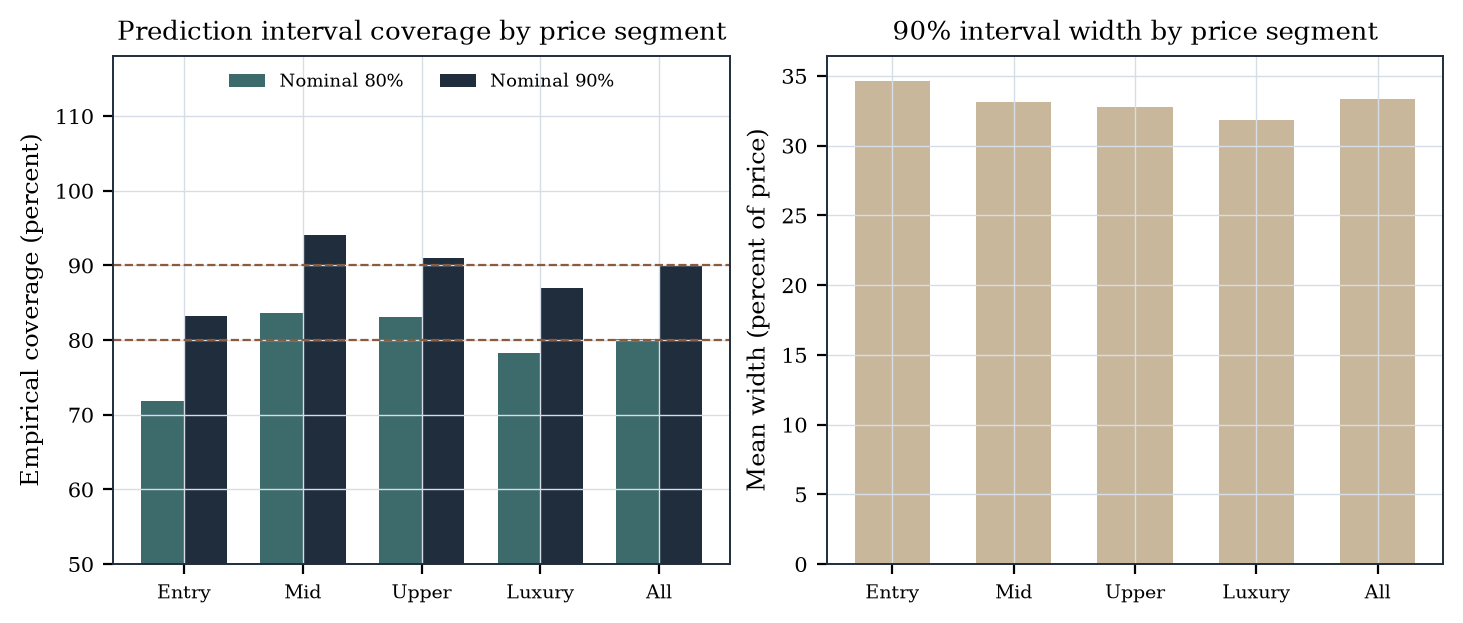
\includegraphics[width=0.88\linewidth]{fig20_interval_coverage.png}
\caption{Empirical coverage of the 80 and 90 per cent conformal intervals by price
band (left) and mean width of the 90 per cent interval as a percentage of price
(right). The entry band under-covers while the mid and upper bands over-cover.}
\label{fig:coverage}
\end{figure}

Figure~\ref{fig:coverage} shows the same pattern graphically. Two caveats accompany
the table. Coverage is measured on the same out-of-fold residuals from which the
quantiles were calibrated, so the overall figures are in-sample for the calibration
step and optimistic as estimates of future coverage; the independent evidence is the
monitoring replay in Section~\ref{sec:monitoring}. And a single global quantile
cannot be correct for both a 90,000 \USD{} starter home and a 500,000 \USD{}
property, because the scale of dollar error differs by a factor of three.
Segment-conditional conformal calibration, or conformalised quantile regression
\citep{romano2019cqr}, would address this and is the highest-value extension of the
uncertainty layer.

\subsection{Residual diagnostics and subgroup performance}

Residual diagnostics are summarised in Figure~\ref{fig:residual}. The mean log residual is $-0.00055$ with a standard
deviation of 0.1112, so the fit is unbiased on average in log space and the typical
multiplicative error is about 11 per cent. The distribution is left-skewed
($-1.141$) and fails the Jarque--Bera test decisively (statistic 2,861, $p<0.001$)
\citep{jarque1980}; the Breusch--Pagan test rejects homoscedasticity (LM statistic
131.9, $p<0.001$) \citep{breusch1979}. Error is also concentrated: the worst five per
cent of cases account for 22.1 per cent of total absolute error, the 90th percentile
of absolute error is 29,122 \USD{} and the maximum is 138,115 \USD. The mean absolute
error of 13,537 \USD{} therefore conceals a tail that matters for escalation
decisions.



\begin{figure}[htbp]
\centering
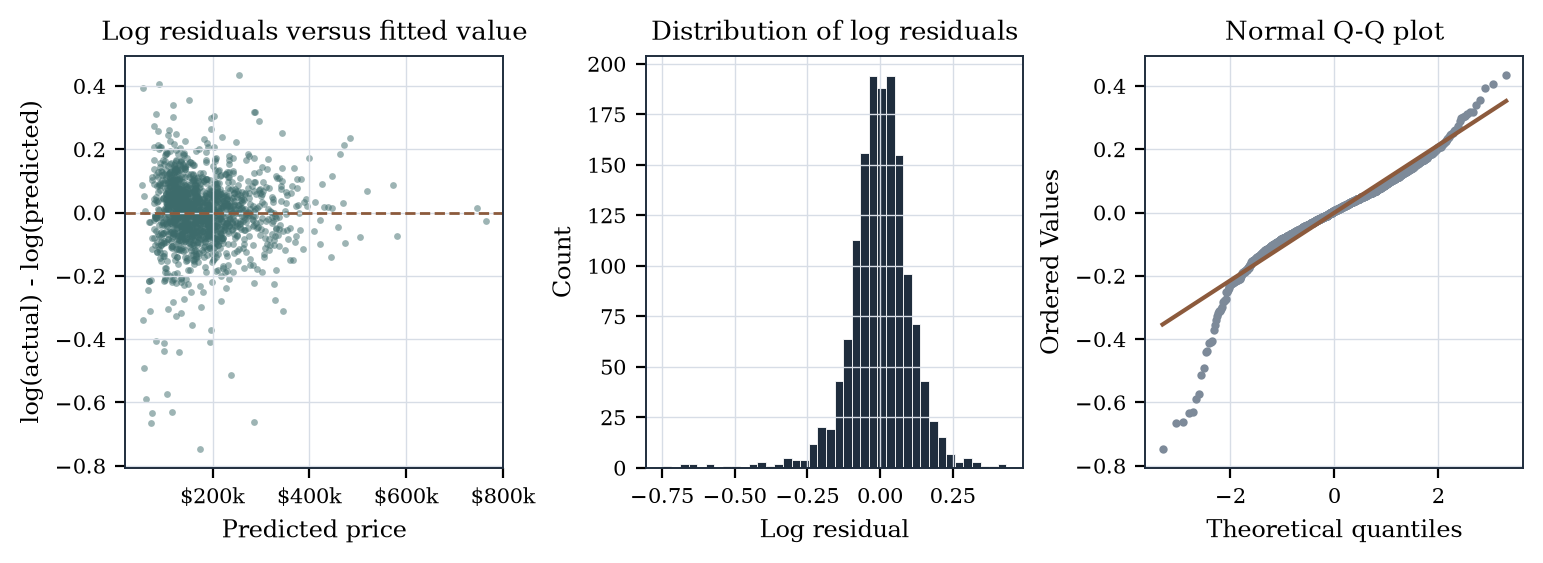
\includegraphics[width=\linewidth]{fig17_residual_diagnostics.png}
\caption{Residual diagnostics: log residuals against fitted value (left),
distribution of log residuals (centre) and normal quantile--quantile plot (right).
The left tail is longer than the right and the quantile plot departs from the
reference line at both ends.}
\label{fig:residual}
\end{figure}

The diagnostics carry three implications. The left skew means the model occasionally
over-predicts substantially, the expensive direction under Equation~\eqref{eq:loss}.
Heteroscedasticity invalidates analytical Gaussian intervals, which justifies the
conformal approach. And the concentration of error means that a product reporting only
the mean would understate the tail risk that drives review decisions.

Table~\ref{tab:subgroup} disaggregates error by neighbourhood segment and price band.
Dollar error rises steeply with price: mean absolute error is 11,581 \USD{} in value
neighbourhoods, 12,892 \USD{} in established neighbourhoods and 23,035 \USD{} in
premium neighbourhoods, and it rises from 10,295 \USD{} in the entry band to 31,238
\USD{} in the luxury band. Relative bias tells the opposite story and is the more
actionable signal. The entry band is over-predicted by 4.70 per cent, so the platform
would systematically quote first-time buyers a price above what they eventually pay,
while the luxury band is under-predicted by 3.92 per cent, transferring value away
from sellers of expensive homes.

\begin{table}[htbp]
\centering
\caption{Subgroup performance of the selected model. Neighbourhood segments group
tiers 1--2 as value, tier 3 as established and tiers 4--5 as premium. Bias is the
mean signed error as a percentage of the sale price; a positive value indicates
over-prediction.}
\label{tab:subgroup}
\small
\begin{tabular}{@{}lrrrr@{}}
\toprule
\textbf{Segment} & \textbf{Sales} & \textbf{RMSE (\USD)} & \textbf{MAE (\USD)} & \textbf{Bias (\%)} \\
\midrule
Value neighbourhoods & 389 & --- & 11,581 & $+1.34$ \\
Established neighbourhoods & 926 & --- & 12,892 & $+0.54$ \\
Premium neighbourhoods & 143 & --- & 23,035 & $+0.08$ \\
\midrule
Entry band ($<$130k) & 365 & 14,521 & 10,295 & $+4.70$ \\
Mid band (130k--200k) & 658 & 15,413 & 10,973 & $+0.08$ \\
Upper band (200k--300k) & 320 & 21,864 & 16,147 & $-0.91$ \\
Luxury band ($\geq$300k) & 115 & 41,499 & 31,238 & $-3.92$ \\
\bottomrule
\end{tabular}
\end{table}

The asymmetry between dollar error and relative bias is the central evaluation
insight of this project. Judged by mean absolute error the model is much worse for
expensive homes; judged by percentage bias it is systematically cheap for expensive
homes and systematically generous for inexpensive ones. Both facts are true and have
different remedies. The first is a scale effect that no model can eliminate entirely,
because expensive properties are heterogeneous and thinly traded. The second is a
calibration defect that segment-specific review thresholds or an asymmetric objective
can address.

\subsection{Drivers of the valuation}

Figure~\ref{fig:shap} ranks the global drivers by mean absolute SHAP value, computed
with the linear explainer for the elastic net and aggregated from one-hot columns
back to their parent attributes \citep{lundberg2017shap}. Rooms above grade
contributes 8.73 per cent of total explanation mass, total floor area 6.51, the
quality--condition index 6.31, average room size 4.51, age at sale 3.41, basement
finish type 3.19, neighbourhood latitude 3.05 and total bathrooms 2.76. Aggregated by
family, structural attributes account for 43.35 per cent, categorical attributes for
27.82, structural composites for 15.87, age and renovation for 6.21, location for
3.20, neighbourhood amenities for 2.40 and macro-financial context for 1.14.

\begin{figure}[htbp]
\centering
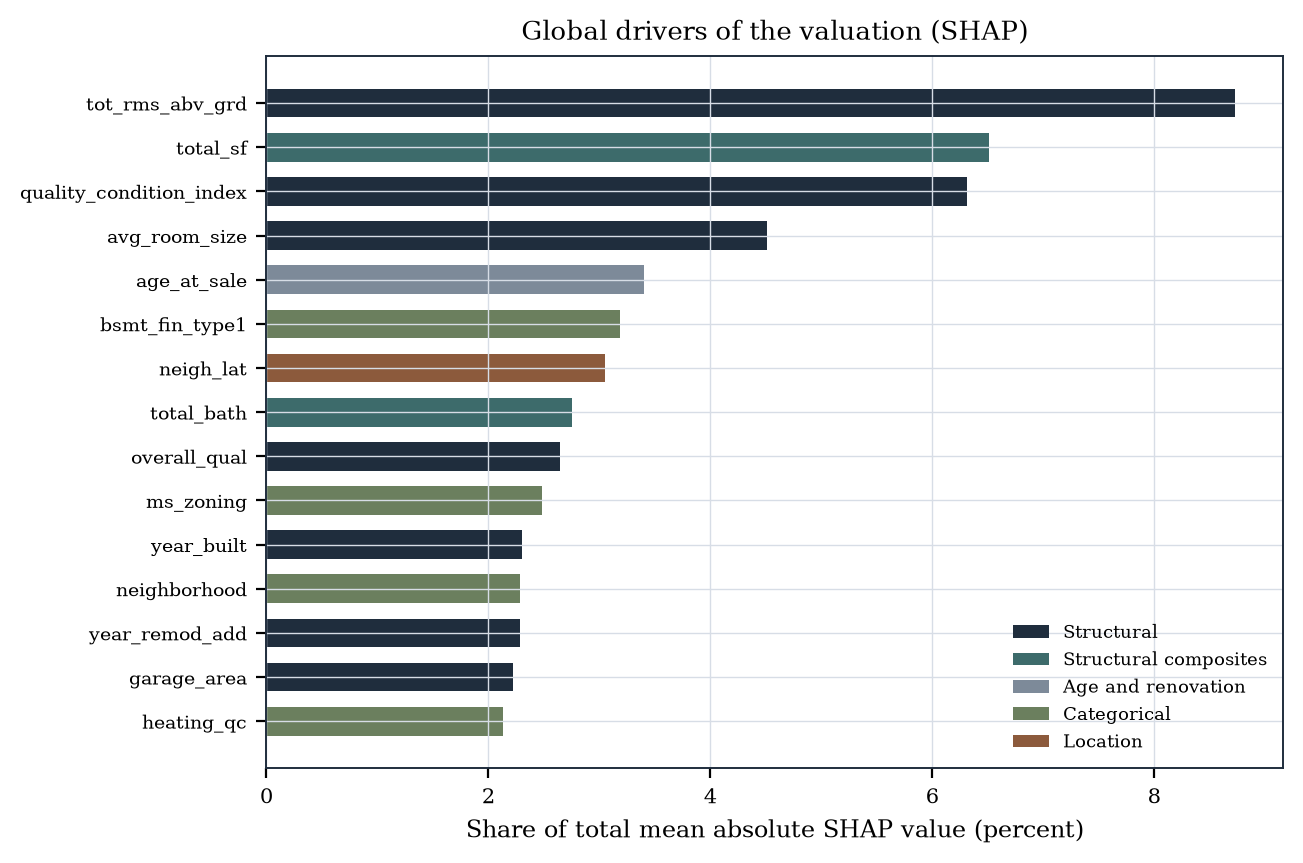
\includegraphics[width=0.74\linewidth]{fig18_global_drivers.png}
\caption{Global drivers of the valuation by mean absolute SHAP value as a share of
the total, coloured by feature family. Structural and categorical attributes
dominate; simulated contextual fields carry a smaller but non-trivial share.}
\label{fig:shap}
\end{figure}

The decomposition supports the business narrative that quality, space and condition
drive value, and it also disciplines it. Location enters indirectly through
neighbourhood indicators and latitude rather than through a single interpretable
premium, and the macro block contributes only 1.14 per cent of in-sample attribution.
That should not be read as evidence that macro conditions do not matter: SHAP values
describe how the fitted model uses each feature across the training distribution,
which contains modest and correlated macro variation. The monitoring
study shows that when the macro block moves outside that distribution, prediction
levels shift and coverage collapses. In-sample attribution and out-of-sample
sensitivity are different questions, and the report keeps them separate.

\subsection{Temporal holdout}

Cross-validation measures interpolation within the sample, not behaviour on future
listings. A temporal holdout provides a stricter test: the model is refitted on the
1,283 sales completed in 2006--2009 and evaluated on the 175 sales completed in 2010,
which are never used for tuning or selection. Root mean squared error rises to 22,269
\USD{} and mean absolute error to 14,820 \USD, with an $R^2$ of 0.9229 and a MAPE of
8.71 per cent. The tolerance hit rate falls to 63.4 per cent and the over-valuation
rate to 36.0 per cent, so the holdout model is both slightly less accurate and
markedly more conservative than the cross-validated one. The 11 per cent degradation
in root mean squared error is the honest estimate of the cost of forecasting forward
in this market, and it remains inside the targets of Table~\ref{tab:kpis}. Part of
the degradation is compositional rather than temporal, because 2010 sales are
concentrated in the first half of the year and the sample is small. The report quotes
the out-of-fold result, the holdout and the monitoring replay rather than the most
flattering of the three.
